\documentclass{article}
\usepackage[utf8]{inputenc}
\usepackage{url}
\usepackage{graphicx}
\graphicspath{ {./} }


\title{Automatisation du prétraitement de photographies de portraits de mandrills}
\author{Maxime Boucher}
\date{Compte rendu 6}

\begin{document}

\maketitle

Nous avions la dernière fois un modèle pour 1FaceQual plutôt moyen, malgré une très bonne précision si l'on accepte une erreur à une classe près (par exemple,
1FaceQual0 et 1FaceQual1) :
\begin{center}
    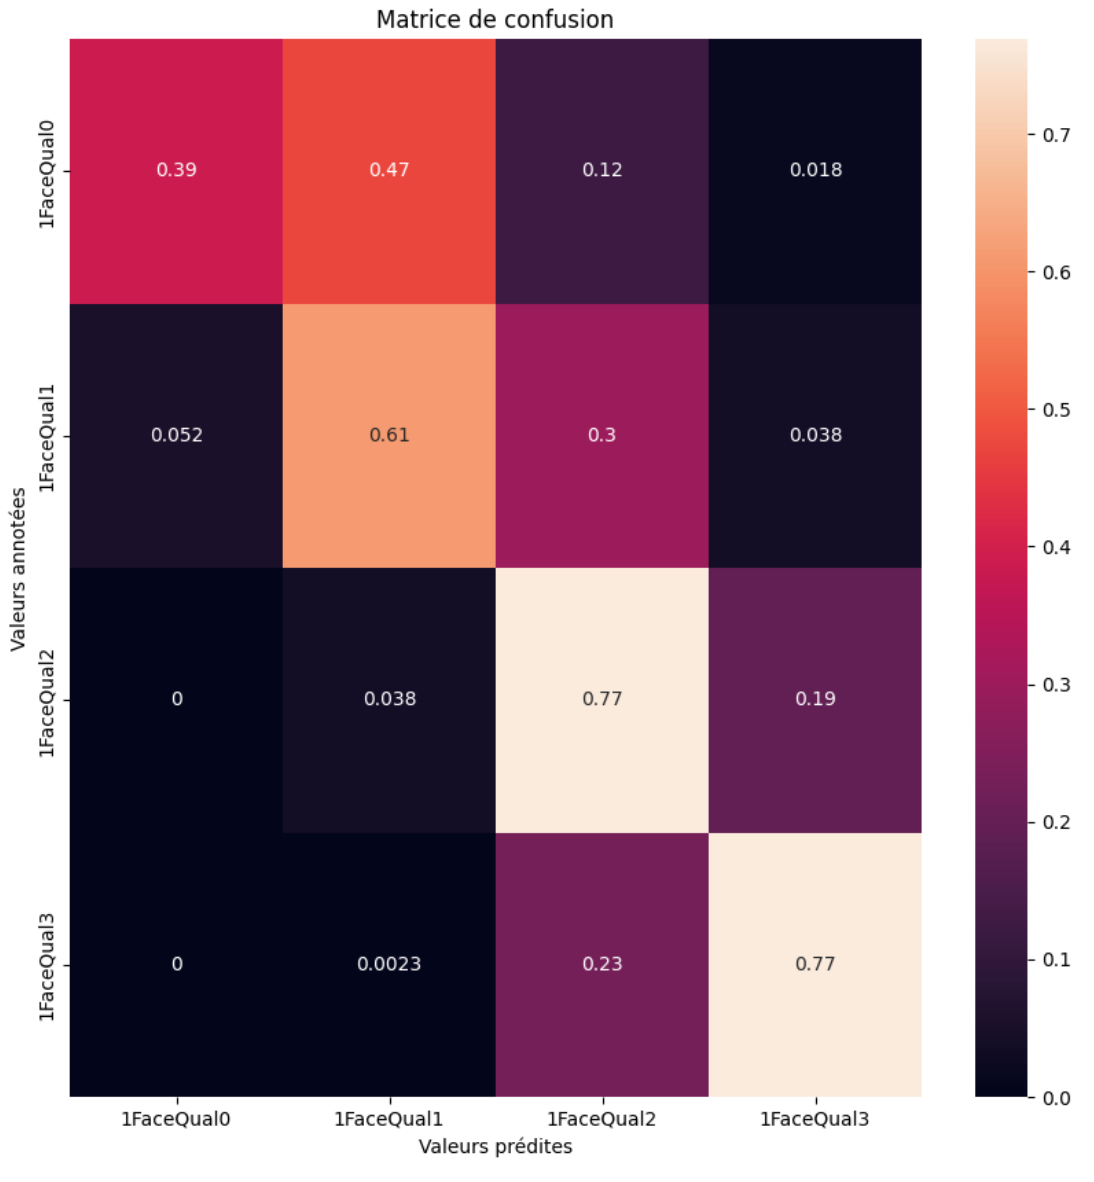
\includegraphics[width=200]{imgs/qualité/cr6/confusion.png}
\end{center}

Pour améliorer ce résultat nous avons essayé de réduire le jeu de données à la période où une seule personne avait annoté les images (en passant donc d'un dataset de 31k images à 19k).
Voici le taux d'échantillons placés : 
\begin{center}
    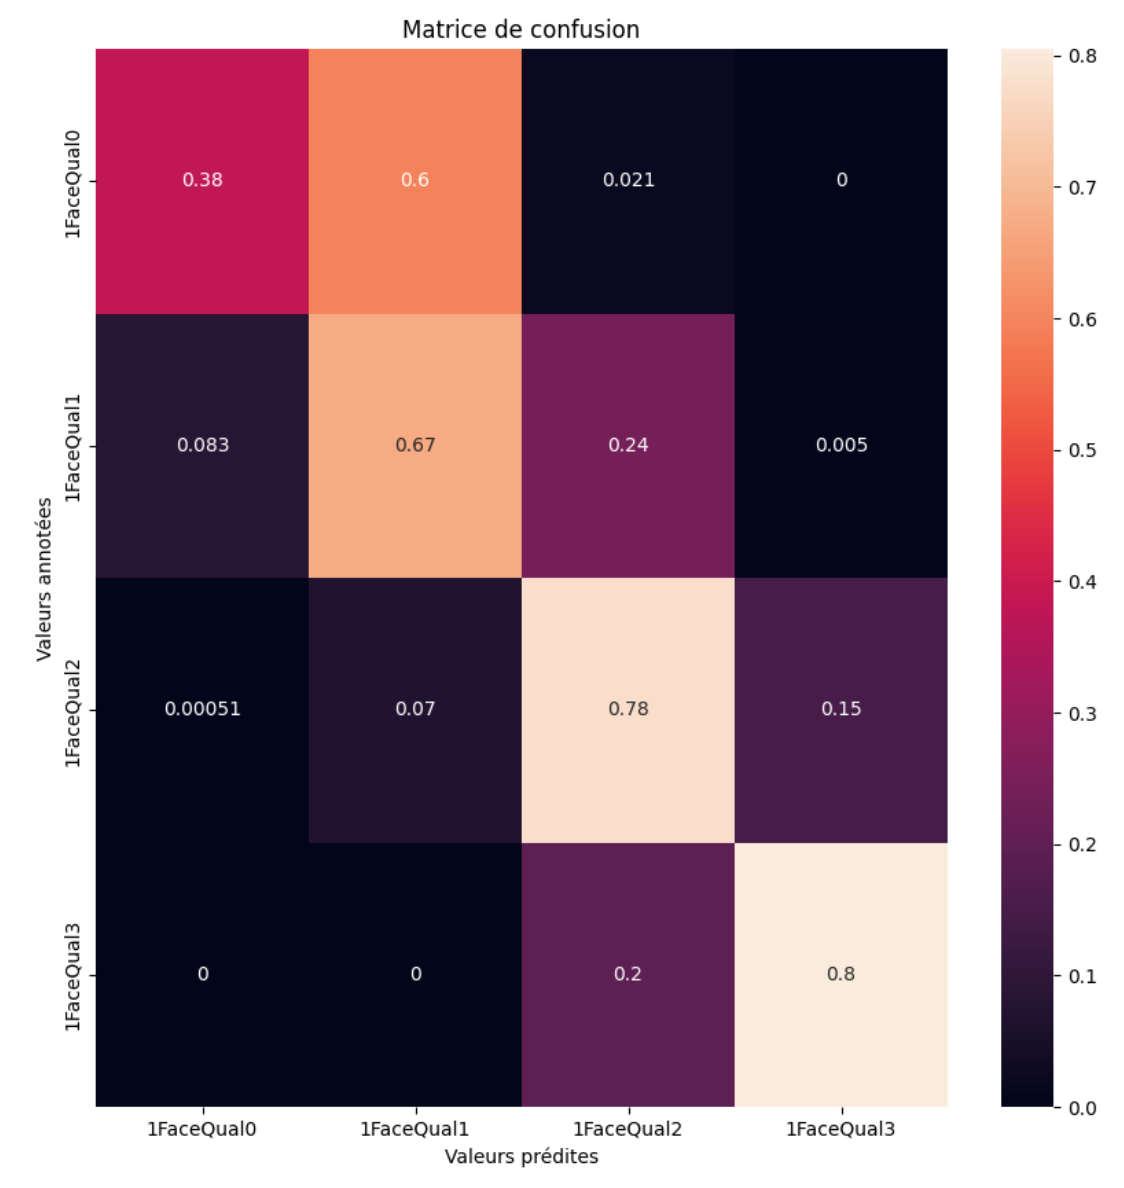
\includegraphics[width=200]{imgs/qualité/cr6/confusion-small.png}
\end{center}

Le résultat n'est cependant pas bien meilleur avec une accuracy moyenne à 0.71 et un écart type de 0.015 en effectuant la stratégie k-fold pour estimer la variance des résultats. J'en déduis que le paramétrage du seed influe peu sur le résultat final (plusieurs "fold" du dataset rendent les mêmes résultats) et donc que réduire le jeu de données n'a pas fonctionné.\\


Pour résoudre ce problème de classification, il est tentant de réduire le problème à une régression, puisque les classes sont corrélés : les classes 1FaceQual0-3 correspondent à une suite d'images de qualité croissante.
Enfin, pour les classifier de manière discrète, il suffirait d'arrondir les prédictions alors continus.
\begin{center}
    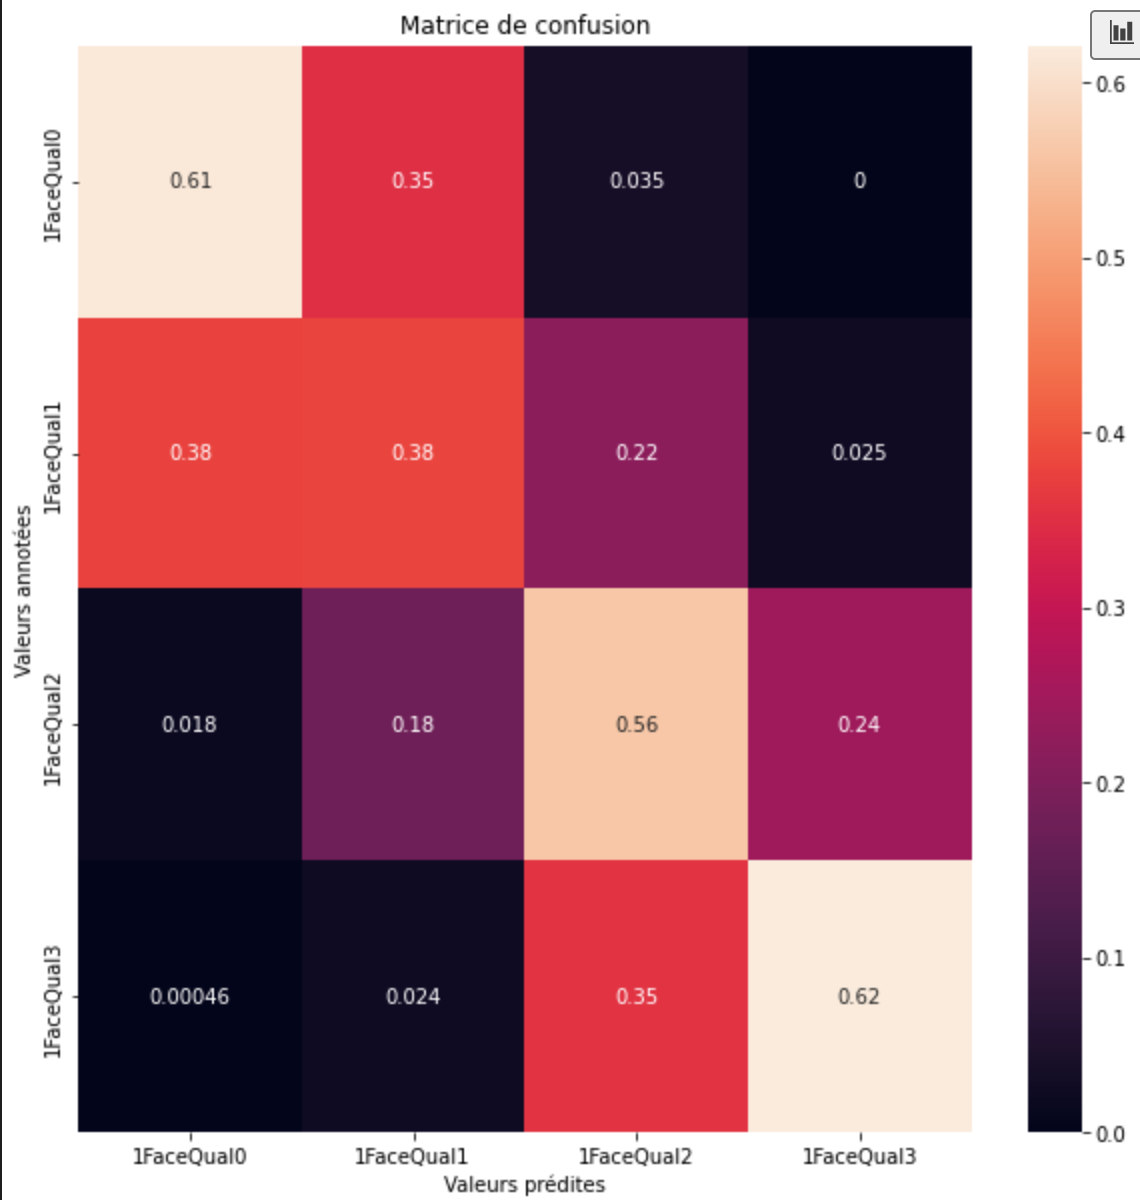
\includegraphics[width=200]{imgs/qualité/cr6/confusion-regression.png}
\end{center}

Le résultat n'est cependant pas aussi bon. Cela est sûrement en partie dû au fait que les valeurs ne sont pas prédites dans l'interval [0; 3] mais [-\infty; +\infty].

On peut supposer affiner les résultats en améliorant les méthodes liés à la normalisation, ou alors en retournant au modèle de classification d'avant avec cross entropy.

\end{document}
